\begin{figure*}
\centering
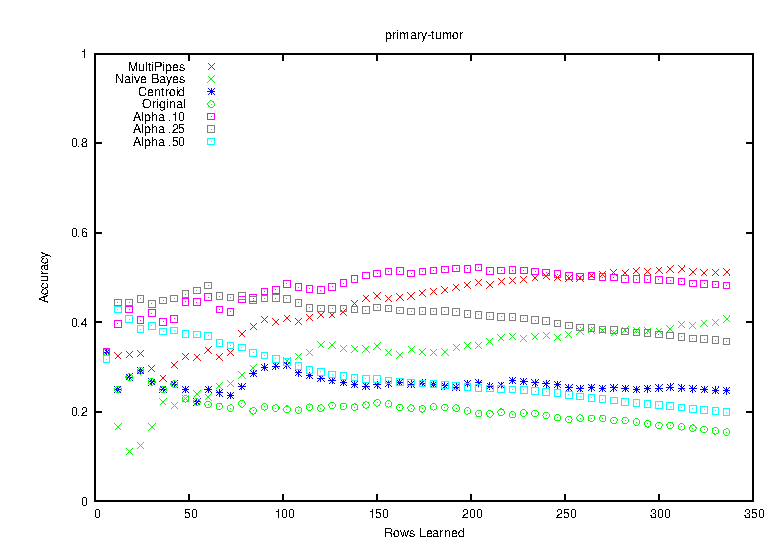
\epsfig{file=charts/primary-tumor.eps}
\caption{Incremental results from a discrete dataset with many class values.}
\label{fig:primary-tumor}
\end{figure*}

Learning with disjoint sets introduces some caveats to data analysis. As seen in figure ~\ref{fig:primary-tumor}, our baseline disjunctive HyperPipes consistently outperforms both naive bayes and the original HyperPipes algorithm. However, our disjuntive learner doesn't exactly play fair, hedgings it's bets with multiple predicted classes. Note as well that when we use our centroid method for single classification, we fail to consistently beat naive bayes.

However, when disjunctive HyperPipes cheats, it does so with a conscious. While the size of the disjunctions varies, on average the set contains only 4 out of 22 possible classes, or about 18\% of the original possible classes. As a result, we trade in single classification for a doubling of accuracy.
